\week{Models v Reality}

Ask an adult and get some modeling clay or Play-doh! and use it to
make a duck.

\begin{marginfigure}
  \centering
  \includegraphics[width=0.8\marginparwidth]{../week2/figures/duck.jpg}
  \caption{Can you make a duck out of Play-doh?}
\end{marginfigure}

Now look at what you made. Is it a duck?

If you're good with your hands and modeling, maybe your creation
really looks like a duck. For others, it might look a bit odd -- maybe
lumpy, maybe missing a wing, or maybe more like a blob than a
bird. But the question is the same for everyone: Is the thing you made
a duck or something else?

In a way, all our models are right. Each model highlights different
parts of what \emph{you} think makes a duck a duck. Maybe you focused
carefully on the beak, or maybe you carefully sculpted feathers for
the wings. There are many details you \emph{could} have included, and the ``right'' choice depends on what you think matters.

This is what it means to make a \emph{model}. A model is not the thing
itself -- it is a simplified version that leaves some things out and
emphasizes others.

Now, imagine being asked to make \emph{one million} ducks. If you
tried making each one by hand the same way you made your first duck,
it would take you a \emph{very} long time. Worse, each duck would
probably come out a little differently. Your hands might get
tired. Your ducks may slowly change.

Instead, you might decide to do something different. You could write
down the \emph{exact instructions} for how to make your duck -- step
by step. Then you could give those instructions to a machine and ask
it to follow them exactly, over and over again. Each duck would then
be made the same way.\didyouknow{Many of the products we use today are
  made by computers that manipulate real life materials, like wood,
  metals, and plastic. Precise instructions are provided to these
  machines using a special computer unit called a \term{Computer
    Numerical Control} (or \term{CNC} module).

  \includegraphics[width=0.8\marginparwidth]{../week2/figures/cnc-machine.jpg}
  % CCBYSA https://upload.wikimedia.org/wikipedia/commons/e/e4/Wheel_Machining.jpg
  }

\begin{TryThisBox}
  Try writing out the \emph{exact} instructions you would give to a
  robot to make a duck, or another simple object. How would you
  describe the object to your robot?
\end{TryThisBox}

This same approach to making things often happens at home. For
example, when you want to make a cake, you first have to look up a
recipe. The recipe is not the cake. You can read the recipe, copy it
or share it, but you can't eat it. Only when you follow the recipe
does a cake appear.  \curious{Here is an interesting question:
  \emph{before anyone bakes the cake, does the cake already exist?} Or
  does it exist only as a description -- a list of instructions --
  waiting to be followed? Philosophers have argued about this for
  thousands of years. Some thought that things like circles, numbers,
  or recipes are real in their own way, even before we use
  them. Others thought that these things only exist because we give
  them names and descriptions. What do you think?}

When writing programs for a computer, we have to consider focusing on
the things that are important for our purposes.

\begin{marginfigure}
  \centering
  \includegraphics[width=0.8\marginparwidth]{../week2/figures/plato.jpg}
  \caption{The Greek philosopher \textbf{Plato} believed that things
    existed before being described.}
\end{marginfigure}

\begin{TrackBox}{Gaming}
  Some computer scientists try to match the descriptions and names on
  the computer match those they observe in the real world. When we do
  this, we can use the computer to predict what would happen. This is
  called a \term{simulation}.
\end{TrackBox}

\section{Re-using models}

The purpose of providing instructions is so that we can do the same
thing over again. Similarly, on a computer, when we write a program
once, we can re-use it many times. Last week, we used the prompt to
immediately process Python rules. This week, we are going to learn how
to set up rules that can be re-used.

The first way to re-use rules is to save them into a \term{file}. We
call rules that we save on a computer \term{source code}.

Let's try saving a rule. Open up Thonny and, instead of the prompt,
point your mouse at the editor
(\prettyref{fig:thonny-interface}). Rules that we type here can be
saved on the computer. Type the following into the editor and then
save it into a file called \texttt{model.py}.
 % TODO add link
\hint{You can also access all these files on the internet}

\begin{TryThisBox}
  Type the following into the editor and then save it in a file named
  \texttt{model.py}.
  \begin{lstlisting}
def three():
<SPACE><SPACE>return 3
def double(x):
<SPACE><SPACE>return x + x
  \end{lstlisting}
\end{TryThisBox}
\hint{From now on, all the rules we see will be
    \emph{colored}. You don't need to enter the colors in. The colors
    only serve to make the rules easier to read. This is called
    \term{syntax highlighting}.}

% TODO describe how to load the file

Now, go to the prompt, and try these rules.

\begin{replbox}
three()<ENTER>
double(3)<ENTER>
double(three())<ENTER>
double(10)<ENTER>
\end{replbox}

What do you see? Did you predict what was going to happen correctly?
Why or why not?

\subsection{Introducing \kw{def} and \kw{return}}

Just like a cake recipe, we can make our own re-usable rules in Python
using the \kw{def} and \kw{return} rules. Here's how it works.

We use \kw{def} to give a \emph{name} to our rules. Then, underneath
\kw{def}, we write the rules that make up the new rule we are
making. The rules underneath have to be \term{indented}, which means
that we have to type two {\spacekey}s before typing the rule.

When Python follows the rules we make, it does \emph{exactly} the
rules we included as part of our named rule, but it doesn't show us
the result of these rules, like what happened when we typed the rules
into the prompt directly. In order to get the final answer from our
named rules, we have to use \kw{return}.

\begin{TryThisBox}
  Type the following into \texttt{model.py}
  \begin{lstlisting}
def three_and_five():
  5
  return 3
  \end{lstlisting}
\end{TryThisBox}

Now try this in the prompt.

\begin{replbox}
three_and_five()<ENTER>
\end{replbox}

\begin{BigIdeaBox}
  We can enter as many rules as we want into \kw{def} but we have
  to use \kw{return} if we want Python to respond with a particular
  rule.
\end{BigIdeaBox}

\subsection{Combining rules}

Remember how \code{+} and \code{*} combined other rules? We can create
our own ways to combine other rules with \kw{def}. First, we have to
give names to the rules that we do not know yet. We can do this by
putting these names in parentheses after \kw{def}.\curious{These names
  for unknown rules are called \term{arguments}, even though there's
  no disagreement. Names can be funny that way!}

\begin{TryThisBox}
  \begin{lstlisting}
def mul_and_add(rule1, rule2, rule3):
  return rule1 * rule2 + rule3
  \end{lstlisting}
\end{TryThisBox}

What do you think will happen if you enter \code{mul\_and\_add(5,2,4)}
into the prompt?
%
\curious{Just like it's important to predict what will
  happen when a rule is used correctly, it's also important to think
  about what happens when rules are used incorrectly. For example,
  what do you think will happen if you entered \code{mul\_and\_add(2)}
  at the prompt?}


Let's think about it. We know what \kw{def} and \kw{return} do. When
we used \code{mul\_and\_add} at the prompt, we gave it three rules:
\code{5}, \code{2}, and \code{4}. If we look at the recipe for
\code{mul\_and\_add} above, we see that it will \kw{return} the
product of the first two rules added to the third one. So, Python's
response will be \code{14}.

We can also say that \code{mul\_and\_add(5,2,4)} \term{evaluates} to
\code{14}. Also, from now on, we will call all the ``recipes'' we make
\term{functions}.

\begin{DeepDiveBox}
  % TODO: The Stack
\end{DeepDiveBox}

\subsection{Complex Rules}

Functions allow us to combine rules. For example, we can use one
function from another. This is known as \term{calling} the function.

By using functions in this way, we can create very complex rule
systems.  \didyouknow{Just like the modeling clay we used at the
  beginning of this class could be used to model any object, we can
  use plain functions to model any system. There's an entire
  discipline of computer science that deals with this idea called
  \term{functional programming}. It's the programmer equivalent of
  playing with Play-doh, but maybe not as messy!}

% TODO introduce calling functions

\section{Drawing with Turtle}

Let's try to apply what we've learned so far by learning how to draw
with Python. As part of the course code, there is a source file named
\texttt{week2/draw.py} which contains a simple \term{library} of
functions that help us make drawings in Python. Let's try using it!

To use a Python library (also called a \term{module}) we use
\kw{import}. In the prompt type:

\begin{replbox}
import week2.draw as draw<ENTER>
\end{replbox}

We can now use functions in the module.
\curious{What do you think would happen if we
  wrote\code{import week2.draw as week2}?
  Would the other code work? How would we have to change the code to
  make it work with this new \kw{import}?}

\begin{replbox}
draw.draw(draw.forward(100))<ENTER>
\end{replbox}

You should see a line on your screen. Congratulations, you've
programmed your first picture!

The drawing system here is based off of an older programming language
called Turtle. Turtle has a few simple rules, which are listed in
\prettyref{tab:turtle}.

But to really understand Turtle, we first have to understand how we
can talk about a computer screen.

\subsection{Introduction to Computer Graphics}

Last week we saw how to use Python to refer to numbers. You've
probably seen the \term{number line} in your math courses. All numbers
can be placed on a simple line, and we can name any point on the line
by writing down a number to name it.
\huh{This coordinate system looks different than
  my math courses! What's going on?}{If you've done geometry you've
  probably seen the cartesian plane drawn with the $y$ coordinate
  increasing as you go up. On many computers, the $y$ coordinate
  increases as you go \emph{down}. Computers often use this different
  coordinate system so that the coordinates match how things are
  physically drawn. It doesn't matter which system you choose, as long
  as everyone does it the same way. In both systems, each grid is
  named by a unique number.}

%\curious{Some mathematicians think
%  there are numbers we cannot quite name. The first person to think of
%  this was a mathematician named \textbf{George Cantor}. If such a
%  number cannot be written, can you think of it? What about write a
%  description of it?}

We cannot draw on a line. We need a rectangle to do that. How do we
name a point on a rectangle? The first person to think about this
systematically was a scientist, mathematician, and philosopher named
\textbf{Ren\'e Descartes} who invented something called the Cartesian
plane. Here's how it works. Instead of a line, we draw a grid. We
number all the columns and all the rows (see
\prettyref{fig:cartesian-grid}). Now, any square on the grid can be
named by giving two numbers. These two numbers together are called the
\term{coordinate}. We usually write the \emph{column} number first,
and the \emph{row} number last. This system is called the
\emph{cartesian coordinate} system.


\begin{figure}[t]
  \label{fig:cartesian-grid}
  \caption{Just like we can refer to any point on a line by a number,
    we can refer to any point on a rectangle or grid using two
    numbers. This is called the cartesian coordinate system. For
    example, in this image of a flower,}
  \centering
  % Requires:
% \usepackage{tikz}
% \usetikzlibrary{calc}

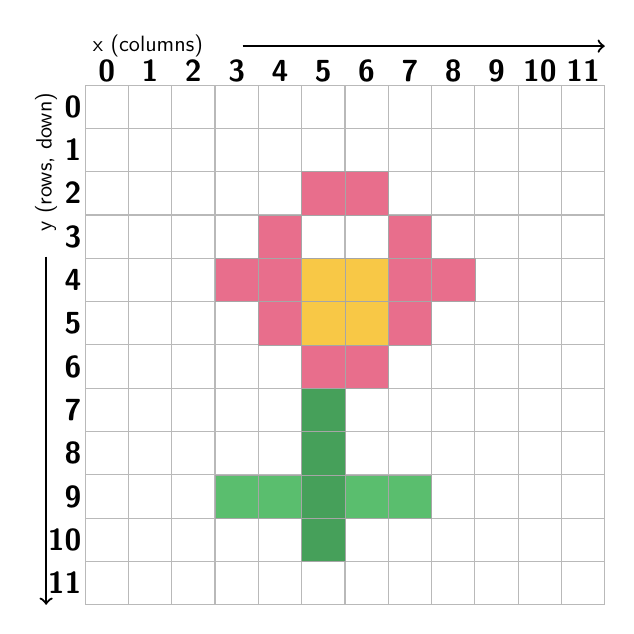
\begin{tikzpicture}[
  font=\sffamily,
  x=0.55cm, y=0.55cm, % pixel size
  line join=round
]
  % ---- grid size ----
  \def\W{12} % number of columns
  \def\H{12} % number of rows

  % ---- background ----
  \fill[white] (0,0) rectangle (\W,\H);

  % ---- draw grid ----
  \draw[step=1, gray!55] (0,0) grid (\W,\H);

  % ---- axis labels: x left->right, y top->bottom ----
  % Column indices along top: 0..W-1
  \foreach \x in {0,...,11} {
    \node[anchor=south, scale=1.1, font=\bfseries\sffamily, inner sep=1pt] at (\x+0.5, \H) {\x};
  }
  % Row indices along left, with y increasing downward:
  % Put 0 at the top row (near y=H-0.5), then 1 below it, ...
  \foreach \y in {0,...,11} {
    \node[anchor=east, scale=1.1, font=\bfseries\sffamily, inner sep=1pt] at (0, \H-\y-0.5) {\y};
  }

  % Optional axis titles
  \node[anchor=west, scale=0.8] at (0, \H+0.9) {x (columns)};
  \draw[->,line width=0.8pt] (2cm, \H+0.9) -s (\W,\H+0.9);
  \node[anchor=east, scale=0.8, rotate=90] at (-0.9, \H) {y (rows, down)}; % name this node Y
  \draw[->,line width=0.8pt] (-0.9, \H+4cm) -- (-0.9, 0); % start this at the south of Y offset by 0.5 downwards and continue it down

  % ---- helper: draw a pixel at (x,y) where y=0 is top row ----
  % We'll just place rectangles manually using the mapping:
  % pixel (x,y) -> rectangle from (x, H-y-1) to (x+1, H-y)

  % Colors
  \definecolor{petal}{RGB}{232,110,140}
  \definecolor{center}{RGB}{248,200,70}
  \definecolor{stem}{RGB}{70,160,90}
  \definecolor{leaf}{RGB}{90,190,110}

  % ---- flower pixels ----
  % petals (a chunky 5x5-ish flower head)


  % Petals (explicit, simpler)
  \foreach \x/\y in {
    5/2, 6/2,
    4/3, 7/3,
    3/4, 8/4,
    4/5, 7/5,
    5/6, 6/6,
    5/4, 6/4, 4/4, 7/4 % make it fuller
  }{
    \fill[petal] (\x, \H-\y-1) rectangle (\x+1, \H-\y);
  }

  % center
  \foreach \x/\y in {5/4,6/4,5/5,6/5} {
    \fill[center] (\x, \H-\y-1) rectangle (\x+1, \H-\y);
  }

  % stem
  \foreach \x/\y in {5/7,5/8,5/9,5/10} {
    \fill[stem] (\x, \H-\y-1) rectangle (\x+1, \H-\y);
  }

  % leaves
  \foreach \x/\y in {4/9,3/9,6/9,7/9} {
    \fill[leaf] (\x, \H-\y-1) rectangle (\x+1, \H-\y);
  }

  % ---- optional: outline the flower pixels slightly darker ----
  \foreach \x/\y in {
    5/2, 6/2,
    4/3, 7/3,
    3/4, 4/4, 5/4, 6/4, 7/4, 8/4,
    4/5, 5/5, 6/5, 7/5,
    5/6, 6/6,
    5/7,5/8,5/9,5/10,
    4/9,3/9,6/9,7/9
  }{
    \draw[black!35, line width=0.2pt] (\x, \H-\y-1) rectangle (\x+1, \H-\y);
  }

\end{tikzpicture}


\end{figure}

\begin{figure}[p]
\begin{TrackBox}{Graphics}
  \emph{Everything} you see on your screen is the result of your
  computer following rules that turn lights on or off (see
  \prettyref{fig:pixels}. Even the text you read is created by
  following rules (known as \term{fonts}) that specify how to turn on
  a pattern of lights to create the letter shapes.

  The drawing library we are using in class translates the functions
  you use into rules that turn on the right lights. Can you think of
  how you might write some rules to draw some of the shapes below?

  \tryitsection

  Here are some problems to think about.

  \begin{enumerate}
  \item Which pixels would you turn on to draw a line between
    coordinate $(5, 2)$ and $(8, 5)$?
  \item What about $(5,2)$ and $(9,0)$?
  \item If someone gave you two coordinates $(x_1, y_1)$ and $(x_2,
    y_2)$ could you come up with a rule that determined which lights
    to turn on to draw a line? Try listing out the instructions
    \emph{exactly}.
  \item Can you use the rule above to draw a triangle?
  \item How would you draw a \emph{circle} around the point $(3, 8)$?
  \end{enumerate}
\end{TrackBox}
\end{figure}

\subsection{Drawing Our First Image}

\begin{table}[t]
  \caption{These are all the Turtle rules you can use and combine
    together using functions!}
  \label{tab:turtle}
  \begin{tabularx}{0.9\linewidth}{ll}
    \toprule
    Rule & What it does\\\midrule
    \code{draw.line} & \\
    \bottomrule
  \end{tabularx}
\end{table}

Turtle works by following -- you guessed it -- rules! Turtle works
like an Etch-a-sketch. You supply instructions that move a pen around
a page. Turtle draws a line as the pen moves. You can also move the
pen without drawing by lifting the pen up, and then restart drawing by
putting the pen down.

Let's try it.

\begin{replbox}
draw.draw(draw.forward(100))<ENTER>
\end{replbox}

What happened here? The pen started in the middle of the page, and
then went \emph{forward} by 100 pixels. In this case, the pen always
starts pointed to the right, so going forward, draws a line to the
right.

Let's try changing the pen color using the \code{draw.color} function.

\begin{replbox}
draw.draw(draw.color('blue')+draw.forward(100))<ENTER>
\end{replbox}

Did it do what you thought it would?

We can even draw a square!
\begin{marginfigure}
  \label{fig:pixels}
  \centering
  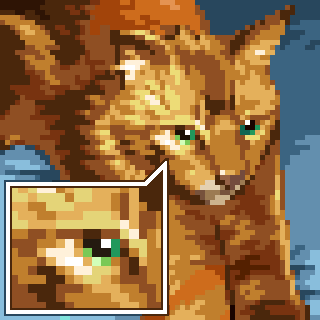
\includegraphics[width=0.9\marginparwidth]{../week2/figures/CatPixels.pdf}
  % CCBYSA4: https://upload.wikimedia.org/wikipedia/commons/7/71/Pixel_Art_Cat_with_Zoom-in_Detail.svg
  \caption{Every image you see on a computer screen is made up of tiny
    lights called \term{pixels} arranged in a grid. By turning the
    lights on and off and adjusting the color, the computer can
    display any image, such as this one of a cat.}
\end{marginfigure}


\begin{replbox}
draw.draw(draw.color('blue') +
  draw.forward(100) +
  draw.turn('right') +
  draw.forward(100) +
  draw.turn('right') +
  draw.forward(100) +
  draw.turn('right') +
  draw.forward(100))<ENTER>
\end{replbox}

Phew! That was a lot of typing! If we had to do that everytime we
wanted to draw a square, we would have to write \emph{a lot} of code.

Let's try writing a function to draw a square. Go to your Thonny
editor and try writing a function to draw a square. It would probably
look like the one below:

\begin{TryThisBox}
  \begin{lstlisting}
def square(n):
  return \<ENTER>
    draw.forward(n) + draw.turn('right') + \<ENTER>
    draw.forward(n) + draw.turn('right') + \<ENTER>
    draw.forward(n) + draw.turn('right') + \<ENTER>
    draw.forward(n)
\end{lstlisting}
\end{TryThisBox}

Let's try using it:
\hint{The \code{\textbackslash} at the end of each line tells Python to treat the
  next line as part of the first. This helps keep our lines shorter
  and easier to read.}

\begin{replbox}
draw.draw(square(100))<ENTER>
\end{replbox}

\mTrackBox{Music \& Sound}{ We've seen how computers represent images as
  lights going on and off, but how do they represent \emph{sound}?

  When our ears hear sound, they are responding to \emph{changes} in
  air pressure.

  Computers represent this -- you guessed it -- using numbers!

  With graphics, we had to break up the rectangular screen into small
  chunks called pixels. For sound, we instead break up \emph{time}
  into really small sections (tens of thousands per second!) called
  samples. Within each sample, we store a number which represents the
  pressure the computer ought to output at that time. When the samples
  are sequenced together rapidly using a componenty called a DAC or
  \term{digital-to-analog converter}. }

You should get something like this:

\includegraphics[width=0.8\linewidth]{../week2/figures/onesquare.eps}

Nice! Now, let's see if we can draw more than one square. We'll also
give our squares some color so that we can tell them apart.

\begin{replbox}
draw.draw(
  draw.color('blue') + square(200) +
  draw.color('red') + square(100))<ENTER>
\end{replbox}

\includegraphics[width=0.8\linewidth]{../week2/figures/twosquares1.eps}

We were able to combine our rules together to draw more than one
square and save us writing twice the amount of code. But hold one, the
second square appeared in a \emph{different} position than the first
one. To understand, let's ask Python to pause before it draws the
squares. Maybe we can figure out what is going on.

\begin{replbox}
draw.draw(draw.pause('square 1') + draw.color('blue') + square(200) + draw.pause('square 2') + draw.color('red') + square(200)
\end{replbox}

When you run this in the prompt, Python will \emph{pause} before each
square is drawn and wait for you to type \enterkey in the prompt
before it continues drawing.  \hint{You can always get back to the
  prompt and quit what you're currently doing by holding down both
  \controlkey and \litkey{C}. This is known as an \emph{interrupt}.}

You should get something like \prettyref{fig:twosquares-debug}.

\begin{figure}
  \label{fig:twosquares-debug}
  \centering
  \begin{minipage}{0.48\linewidth}
    \centering
    \includegraphics[width=\linewidth]{../week2/figures/twosquares-debug-square 1.eps}\\
    The First Square
  \end{minipage}
  \hfill
  \begin{minipage}{0.48\linewidth}
    \centering
    \includegraphics[width=\linewidth]{../week2/figures/twosquares-debug-square 2.eps}\\
    The Second Square
  \end{minipage}
  \caption{What it looks like before each square is drawn. Can you
    spot the difference?

    \textbf{Hint:} Look at the arrow.}
\end{figure}


What do you notice about the arrow? In Turtle, this arrow is called
the \emph{cursor} and its direction changes how \code{draw.forward}
works. If the arrow is pointing right, then \code{draw.forward} draws
to the right. Similarly, if the arrow is pointing towards the top,
then \code{draw.forward} draws towards the top. If you look at the
arrow, you'll notice that, before the first square, it points right,
and before the second, it points upward.

How do we fix this issue? The cursor starts pointing right by
default. It points upward after the first square is drawn using the
\code{square} function. How do we get it to point right again? Can you
think of an answer?

\begin{BigIdeaBox}
  Sometimes, when combining programs together, things don't work the
  way we expect because our mental model of how the computer ought to
  have done something doesn't match the exact set of rules the
  computer followed.

  It often helps to use tools like \code{draw.pause} to inspect what
  is happening in the middle of our program. This is called
  \term{debugging}.
\end{BigIdeaBox}

Here's the solution (pay attention to the italicized part!)

\begin{TryThisBox}
  \begin{lstlisting}
def square(n):
  return \
    draw.forward(n) + draw.turn('right') + \
    draw.forward(n) + draw.turn('right') + \
    draw.forward(n) + draw.turn('right') + \
    draw.forward(n)@@ + draw.turn('right')@@
  \end{lstlisting}
\end{TryThisBox}

Now, our squares are drawn the same way, but they overlap:

\includegraphics[width=0.8\textwidth]{../week2/figures/twosquares-fixed.eps}

There's only one problem now, which is that our squares all start at
the same spot. Can we move them? The answer is yes, using \code{draw.goto}.

\begin{replbox}
draw.draw(draw.color('blue') + square(200) + \<ENTER>
  draw.goto(50,50) + draw.color('red') + \<ENTER>
  square(100))<ENTER>
\end{replbox}

\subsection{A More Complicated Example}

Squares and lines are interesting, but it would be hard to do a lot of
interesting drawing using just those. Let's look at some other shapes.

The first shape we'll introduce is a \emph{circle}. A circle is defined by its radius, which is half the total distance across the circle. For example, to draw a circle with a 30 unit radius, we can use \code{draw.circle(30)}. Try this and see what happens.

\begin{replbox}
  draw.draw(draw.circle(30))
\end{replbox}

But there's more, you can also draw \emph{parts} of a circle. This is
called an \emph{arc}. To draw an arc, you can use
\code{draw.circle(30, 1/2)}, which will only draw \emph{half} the
circle\hint{You can use \code{1/2} or \code{0.5}. Python understands
  both.}

\begin{replbox}
draw.draw(draw.circle(30, 0.5))<ENTER>
draw.draw(draw.circle(40, 1))<ENTER>
draw.draw(draw.circle(20, 1/3))<ENTER>
\end{replbox}

Now, try drawing this figure.

\includegraphics[width=0.5\textwidth]{../week2/figures/lrcircle.eps}

Having trouble? Think back to the examples we tried above. Which way
did the arrow move when drawing the circle?

Turtle assumes that when we want a circle, we always want to draw it
in this direction (counter-clockwise). To make it draw in a clockwise
direction, we supply it a \emph{negative} radius. This arrangement
where a computer system always does things one way and requires the
programmer to explicitly choose another way is called a
\term{default}.

To draw the diagram, use this code:

\curious{Try using \code{draw.pause} to visualize exactly which
  portion is drawn by which command!}
\begin{replbox}
draw.draw(draw.circle(30, 1/2) + draw.circle(-30, 1/2))
\end{replbox}

With these shapes, we can make more complicated figures. There's just
one thing left: adding color.

We saw how to change the color of the lines we drew, but how do we
\emph{fill} the shapes we draw with a color?

The \code{draw} module provides the \code{draw.fill} rule to create
filled diagrams. Let's try it.

\begin{replbox}
draw.draw(draw.fill('blue', draw.square(100)))<ENTER>
\end{replbox}

\section{The Duck Challenge}

Remember how we built that duck out of play-doh at the beginning of
the class? Everyone chose different things to focus on. Now it's time
to teach a computer to do what you did.

\begin{TryThisBox}
  Try using what you've learned thus far to draw a duck using \kw{def}
  and \kw{return} and Turtle. Name your function \code{duck}.

  As you're doing this, try to keep re-usable parts of your duck in
  separate functions, so you don't have to copy the code.
\end{TryThisBox}

Here are some examples of what you may have created. All of these are
examples of a ``duck'' that you can make using the simple rules for
drawing we learned above.

\begin{BigIdeaBox}
  To the computer, there is no duck. It's just a set of rules you told
  it to follow to draw one depiction of a duck that you found
  useful. All computer programming requires us to understand the
  problem we're trying to solve.
\end{BigIdeaBox}

\section{Copying Ducks}

You've now drawn \emph{one} duck; what if we wanted more? The whole
point of this was to codify exactly how to make a duck and explain
that to the computer. Now, with these instructions in hand, we can
make more ducks. Let's get started.

\begin{replbox}
from week2.examples import *<ENTER>
lake_of(duck)
\end{replbox}

Nice! Look at all those ducks. But, there's one problem... all our
ducks look the same. Can we make each one a bit more unique?

Let's add some \term{arguments} to our \code{duck} function. Modify
your function to include some arguments.
\begin{TryThisBox}
  \begin{lstlisting}
def duck(@@body_color@@, @@eye_color@@):
  @@your code@@
  \end{lstlisting}
\end{TryThisBox}

Now, take these arguments and use it to change your duck's body and
eye color using the \code{draw.color} and \code{draw.fill} functions
we saw above.

Now, rerun the example above:

\begin{replbox}
from week2.examples import *<ENTER>
lake_of(duck)
\end{replbox}

Much better!

\begin{BigIdeaBox}
  Since we packaged our duck into a function and added arguments to
  allow certain parts to change, we made it trivial to re-use our duck
  many times. This is a foundational part of computer programming.
\end{BigIdeaBox}

\section{Conclusion: From Drawing to Computation}

In this lesson we learned that we can often do things by hand that
take effort to describe to the computer. But once we undertake that
effort, we can use the computer to simulate things that we could not
do by hand. By expressing our duck as sets of numerical rules, we
could hand it to a computer -- a machine that follows rules -- and
manipulate it in new ways. Even though the computer couldn't
\emph{understand} the duck, it could still do useful things with our
description.

Everything in computer science is a description of something real
(whether a physical item or a real problem) that we want to solve. To
be able to manipulate this thing with computers we have to be able to
express our problem as rules the computer understands. In the case of
visual information, it means understanding graphics like the Turtle
system. In the next chapters, we'll explore other ways of describing
the world to a computer.

\Exercises

\begin{exercises}
\item Try creating some other animal as a Python function, and using
  it with the \code{lake\_of} function we used before. What does this
  show about Python's \emph{understanding} of the thing we drew?
  \answer{Whichever animal we draw, Python and the lake\_of
    function treat it the same way. Each animal is just a rule
    for Python to draw.}

\item Can you think of how the \code{lake\_of} function is able to make
  our simple image appear as if it were moving? Are there any rules
  that would create the animation sequence of each duck?

  \answer{TODO}
\end{exercises}

% Show red and blue yin/yan thing
% # ============================================================
% # Chapter 2 TODO Outline (Technical-first)
% # ============================================================
% 
% * Drawing Primitives (Missing Technical Core) - Done
% - Introduce arcs / circles as drawing primitives - Done
% - Show how arcs differ from straight lines - Done
% - Explain radius + angle intuitively (no formulas yet) - Need to ADD diagram
% - Add example: combining lines + arcs -- NOT DONE
% - Add figure showing arc parameters visually -- TODO
% 
% * Filling and Regions -- DONE
% - Introduce closed shapes -- TODO
% - Explain what ?inside? vs ?outside? means -- TODO
% - Introduce fill as coloring a region - DONE
% - Show same outline with and without fill - Add diagram TODO
% 
% * Multiple Duck Representations (Technical)
%     - Draw duck using only lines
%     - Draw duck using lines + arcs
%     - Draw duck using fill
% - Compare versions side-by-side
% - Ask: what details were added / removed?
% 
% * Modeling Choices -- will not do
% - Explicitly name ?model? at this point
% - Identify what each duck drawing ignores -- figure caption
% - Identify what each drawing keeps -- figure caption
% - Add diagram: same duck, different models
% 
% * Simulation: A Lake of Ducks
% - Introduce idea of many ducks, same rules -- done
% - Add simple rule-based placement (position, size, direction)
% - Show variation via parameters -- done
% - Simulate multiple ducks on a lake
% - Add figure: single duck vs many ducks
% 
% * Abstraction via Parameters -- colors of body, and eyes
% - Name parameters explicitly -- 
% - Show how changing numbers canges appearance -- TODO
% - Connect parameters to ?knobvs? on the model -- no
% 
% * From Drawing to Computation
% - State: computer draws by following rules
% - Emphasize repeatability
% - Emphasize no understanding of ?duck?
% 
% * Curiosity / Track Boxes (Insert Where Natural)
% - Graphics: circles aren?t really circles
% - Games: fake physics
% - Sound: sound as numbers
% - Simulation: same rules, many agents
% 
% * Conceptual Wrap-Up
% - Revisit duck question one last time
% - State: model ? thing
% - State: computers work only with models
% - End with forward-looking question
% 
% # ============================================================
